\section{La hidrografía de Andalucía}

\subsection{Los ríos andaluces}

Los ríos de nuestra comunidad (Figura \ref{fig:rios-andaluces}) son cortos, poco caudalosos y de régimen irregular. Unos desembocan en el océano Atlántico, y otros, en el mar Mediterráneo.

\begin{figure}[!ht]
    \centering
    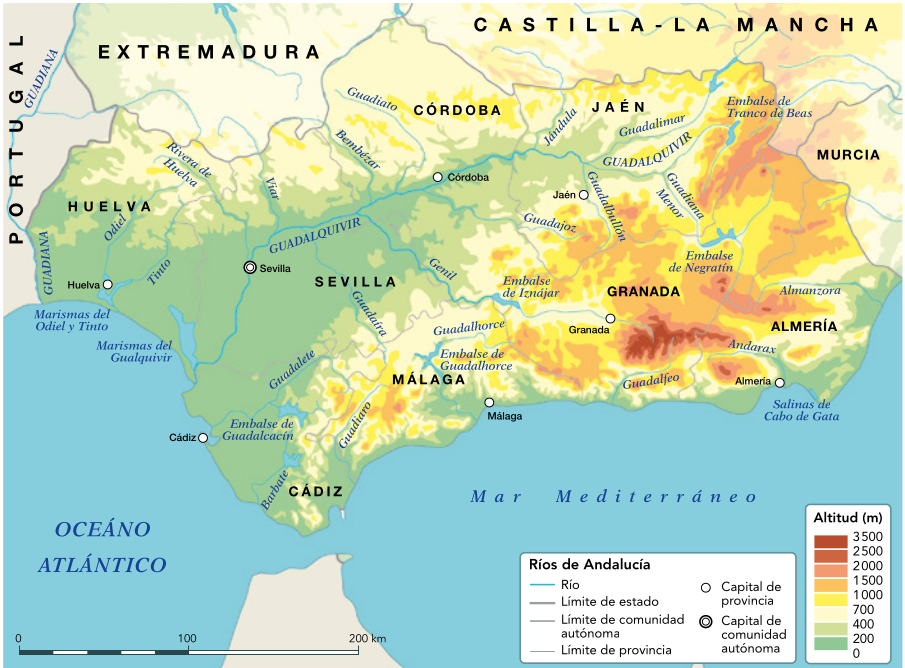
\includegraphics[width=1\linewidth]{Tema2/09_Rios_andaluces.png}
    \caption{Ríos andaluces}
    \label{fig:rios-andaluces}
\end{figure}

\subsubsection{Los ríos de la vertiente atlántica}

Los ríos de esta vertiente son los más largos y caudalosos de la comunidad, su régimen es irregular. Destacan el Barbate, el Tinto, el Odiel, el Guadalete, el Guadiana y el Guadalquivir.

\begin{itemize}
    \item El \textbf{Guadiana} nace en la provincia de Ciudad Real y desemboca en Ayamonte (Huelva), formando frontera con Portugal.
    \item El \textbf{Guadalquivir} es el río más largo e importante de Andalucía. Nace en la sierra de Cazorla, en la Cañada de las Fuentes, en Quesada (Jaén). Atraviesa las provincias de Jaén, Córdoba, Sevilla, desde donde es navegable hasta su desembocadura, en Sanlúcar de Barrameda (Cádiz), tras recorrer 580 km. Sus principales afluentes son el Guadiamar, el Jándula, el Genil, el Guadiana Menor y el Guadajoz.
\end{itemize}

En muchos de estos ríos se han construido embalses, como el de Tranco de Beas, en el Guadalquivir, y el de Iznájar, en el Genil.

\subsubsection{Los ríos de la vertiente mediterránea}

Los ríos que desembocan en el Mediterráneo nacen en la cordillera Penibética. Son \textbf{ríos cortos} y su \textbf{caudal es escaso y muy irregular}. Los más importantes son el Guadiaro, el Guadalhorce, el Guadalfeo, el Andarax y el Almanzora. En estos ríos hay embalses, como el de Negratín, en el Guadiana Menor, y el embalse de Guadalhorce.

\subsection{Las lagunas y los humedales}

Andalucía cuenta con un \textbf{gran número de lagunas y humedales}, que conforman ecosistemas en el que conviven especies protegidas tanto de flora como de fauna. El origen de estos ecosistemas es muy variado:

\begin{itemize}
    \item Sin salida al mar, como las lagunas de Zóñar y Tíscar en Córdoba, de Fuente de Piedra en Málaga y Salinas de Cabo de Gata en Almería.
    \item Creados por la intervención humana, como Laguna Grande en Jaén o el embalse de Malpasillo y Cordobilla, entre las provincias de Córdoba y Sevilla.
    \item \textbf{Marismas}, formadas en la desembocadura de los ríos Odiel y Tinto en Huelva y en la del río Guadalquivir en Sanlúcar de Barrameda (Cádiz). Estas marismas se adentran hasta varios municipios de la provincia de Sevilla, formando parte del Parque Natural de Doñana.
\end{itemize}